\documentclass{acm_proc_article-sp}
\usepackage[utf8]{inputenc}
\usepackage{times}
\usepackage{url}
\usepackage{latexsym}

\usepackage{makecell}
\usepackage{pbox}
\usepackage{color}
\usepackage{graphicx}
\usepackage{csquotes}

\begin{document}
\title{Linghub: Aggregated Metadata about Language Resources as Linked Data}

\numberofauthors{2} 
\author{
\alignauthor
John P. McCrae\\
       \affaddr{CIT-EC, Bielefeld University}\\
       \affaddr{Bielefeld, Germany}\\
       \email{jmccrae@cit-ec.uni-bielefeld.de}
\alignauthor
Philipp Cimiano\\
       \affaddr{CIT-EC, Bielefeld University}\\
       \affaddr{Bielefeld, Germany}\\
       \email{cimiano@cit-ec.uni-bielefeld.de}
   }

\maketitle
\begin{abstract}
    Language resources are an essential component of any natural language
    processing system and such systems can only be applied to new languages and
    domains if appropriate resources can be found. Currently the task of finding
    new language resources is complicated by the fact that their records are
    stored in different repositories with different models, different quality
    and search mechanisms. We present Linghub a new portal that aggregates data
    from a range of sources and uses linked data to make them available under a
    common interface. Furthermore, we use facetted browsing and SPARQL query to
    show how this can help to answer real user problems extracted from a mailing
    list for linguists.
\end{abstract}

\section{Introduction}

Language resources are essential for nearly all tasks in natural language
processing (NLP) and in particular
for the adaptation of resources and methods to new domains and languages. In
order to use language resources for new purposes they must first be discovered
and this can only be done if there is a comprehensive list of all resources that
may be available. To this there have been a number of projects that have
attempted to collect such a catalogue using various methods and with differing
degrees of data quality. We present a new portal, Linghub, that aims to integrate all
these data from different sources by means of linked data and thus to create a
portal, whereby all information about language resources can be included and
queried using a common methodology. As such, this resource will enable wider
discovery of language resources for researchers in NLP, computational
linguistics and linguistics.

Currently, the approaches to metadata collection can be split into two broad
classes: firstly, \emph{curatorial} resources, which are those for which collections of
language resources are maintained by one or more institute. Such resources have
an advantage in that such metadata is normally of very high quality, however the
resulting data often fails to cover the whole spectrum of data available.
Examples of this include the META-SHARE~\cite{federmann2012meta} project and the
CLARIN project's Virtual Language Observatory~\cite[VLO]{van2012semantic}. On
the other hand, \emph{collaborative} approaches rely on data publishers
self-reporting data about their own language resources. This can be advantageous
as it allows reporting by researchers not directly collected to existing
infrastructure projects, however the resulting data is often of lower quality as
the systems may use free-text input or tagging input rather than controlled
vocabularies, as they are easier for non-expert users to understand.

Given the nature of this difference we wish to make data available from multiple
sources in a homogeneous manner and to this end we adopted a model based on the
DCAT data model~\cite{maali2014data} along with properties from Dublin
Core~\cite{weibel1998dublin}. In addition, we used the RDF
version~\cite{mccrae2015ontology} of the META-SHARE
model~\cite{gavrilidou2012meta}, to provide for metadata properties that are
specific to language data and linguistic research. As such, in this paper we
describe the creation of the largest collection of information about language
resources and briefly describe its publication on the Web by means of linked
data principles.

The rest of the paper is structured as follows...

\section{Related Work}

There have been several attempts to collect metadata about language resources
mostly associated with large infrastructure projects. CLARIN has been collecting
resources under a project called the Virtual Language
Observatory~\cite{van2012semantic}, using the Component
Metadata Infrastructure~\cite[CMDI]{broeder2012cmdi} to collect common metadata
values from multiple sources. A similar project is
META-SHARE~\cite{piperidis2012meta} from the META-NET project where language
resources are collected and high-quality, manual entries are created for each
record. Similarly, the Open Languages Archives
Community~\cite[OLAC]{bird2003extending} collects data from a number of sources
although the metadata collected is not itself open. A similar project called
SHACHI has also collected some metadata~\cite{tohyama2008shachi}. There has also
been an attempt to track language resources by means of assigning them an
International Standard Language Resource Number (ISLRN) similar to an ISBN used
to track books~\cite{choukri2012using}.

On the contrary some resources have instead collected data directly from
creators of the resources, for example the LRE-Map~\cite{calzolari2012lre} collects data from
authors of papers submitted to conference, such as LREC. Similarly,
Datahub~\footnote{\url{http://datahub.io}} collects resources directly from
those submitted to the website, but focusses primarily on linked data resources.

\section{Dataset}

\begin{table}
	\centering
	\begin{tabular}{p{30mm}|cc}
	Source               & Records    & Triples  \\
	\hline
	Datahub              & 185        & 10,739   \\
	LRE-Map              & 682        & 10,650   \\
	META-SHARE           & 2,442      & 464,572  \\
	CLARIN VLO           & 144,138    & 3,605,196\\
	\hline
	All                  & 147,447    & 4,091,157\\
	\end{tabular}
	\caption{Size of Linghub dataset by source\label{tab:size}}
\end{table}

In order to ensure that all the data from many sources can be queried in a
homogenous manner we had to convert them to RDF. This process is also proved to
be a valuable opportunity to align these vocabularies with standard vocabularies
and fix any modelling errors. Two of our resources, LRE-Map and Datahub, were already available in RDF
and thus, it should be the case that that the conversion of these resources
required only renaming the URLs so that they would resolve without any
collisions when uploaded to the Linghub portal. In fact, we also took this
opportunity to fix a number of quality issues, such as fixing property values to
either literals or URIs, reducing the number of blank nodes and changing
modelling to that recommended in relevant standards, such as
VOID~\cite{alexander2011describing}. 

The other resources used XML schemas, for which we needed to create a custom
conversion for each of them, which we did with the help of an invertible
transformation language similar to XSLT. For META-SHARE, this was a challenging
task as there were nearly a thousand unique tags defined and each one was
examined to see if it was similar to an existing Semantic Web vocabulary, and in
fact we ended up mapping to FOAF~\footnote{\url{http://xmlns.com/foaf/spec/}},
SWRC~\footnote{\url{http://ontoware.org/swrc/}} and the Media
Ontology~\footnote{\url{http://www.w3.org/TR/mediaont-10/}}. In the case of
CLARIN, there was actually a significant difference between the XML schemas used
by each contributing instance, with only a small common section giving the
resource title and download link. We thus developed distinct mappings for the
largest X institutes.

%\begin{table*}
%	\centering	
%	\begin{tabular}{p{50mm}p{50mm}|cc}
%	Property     & Target             & Links        \\
%	\hline
%	Language     & LexVo              & 92,717       \\
%	Type         & BabelNet           & 12,139       \\
%	Usage        & META-SHARE OWL     & 1,310        \\
%	Rights       & License Ontology   & 103          \\
%	Backlink     & Original Resources & 146,765      \\
%	\end{tabular}
%	\caption{Number of introduced links in the Linghub data\label{tab:links}}
%\end{table*}	

Two key issues emerge when collecting data from a heterogenous set of sources 
such as we are doing. Firstly, the data is likely to be noisy and inconsistent 
in the properties it uses and more importantly in the values that these
properties have. For example, languages may be represented by their English 
names or alternatively by means of the codes such as the ISO 639 codes. Secondly,
it is often the case that a dataset may be recorded in multiple sources and thus,
we may create multiple records of the same dataset. Furthermore, we often see
duplication in the form of multiple records describing different sections of a 
single dataset or multiple usages of the single dataset. In order to remove 
these duplications we used state-of-the-art word sense disambiguation techniques, 
including Babelfy~\cite{Moroetal:14tacl} to identify common controlled vocabularies and duplicate
entries. For the case of properties we mapped to several existing resources, 
including LexVo~\cite{de2013lexvo} for languages, and BabelNet for resource types. Duplicate 
entries were not removed from the dataset but instead were marked with the addition
of the Dublin Core property \emph{is replaced by}. In the case that these entries
were subsets of resources the target of this link would be a new combined record
for the entire resource and in the case of duplicate records collected from distinct
sources we referred to the most complete triple, that is the record with the most
triples.

\section{The Linghub portal}

\begin{figure*}
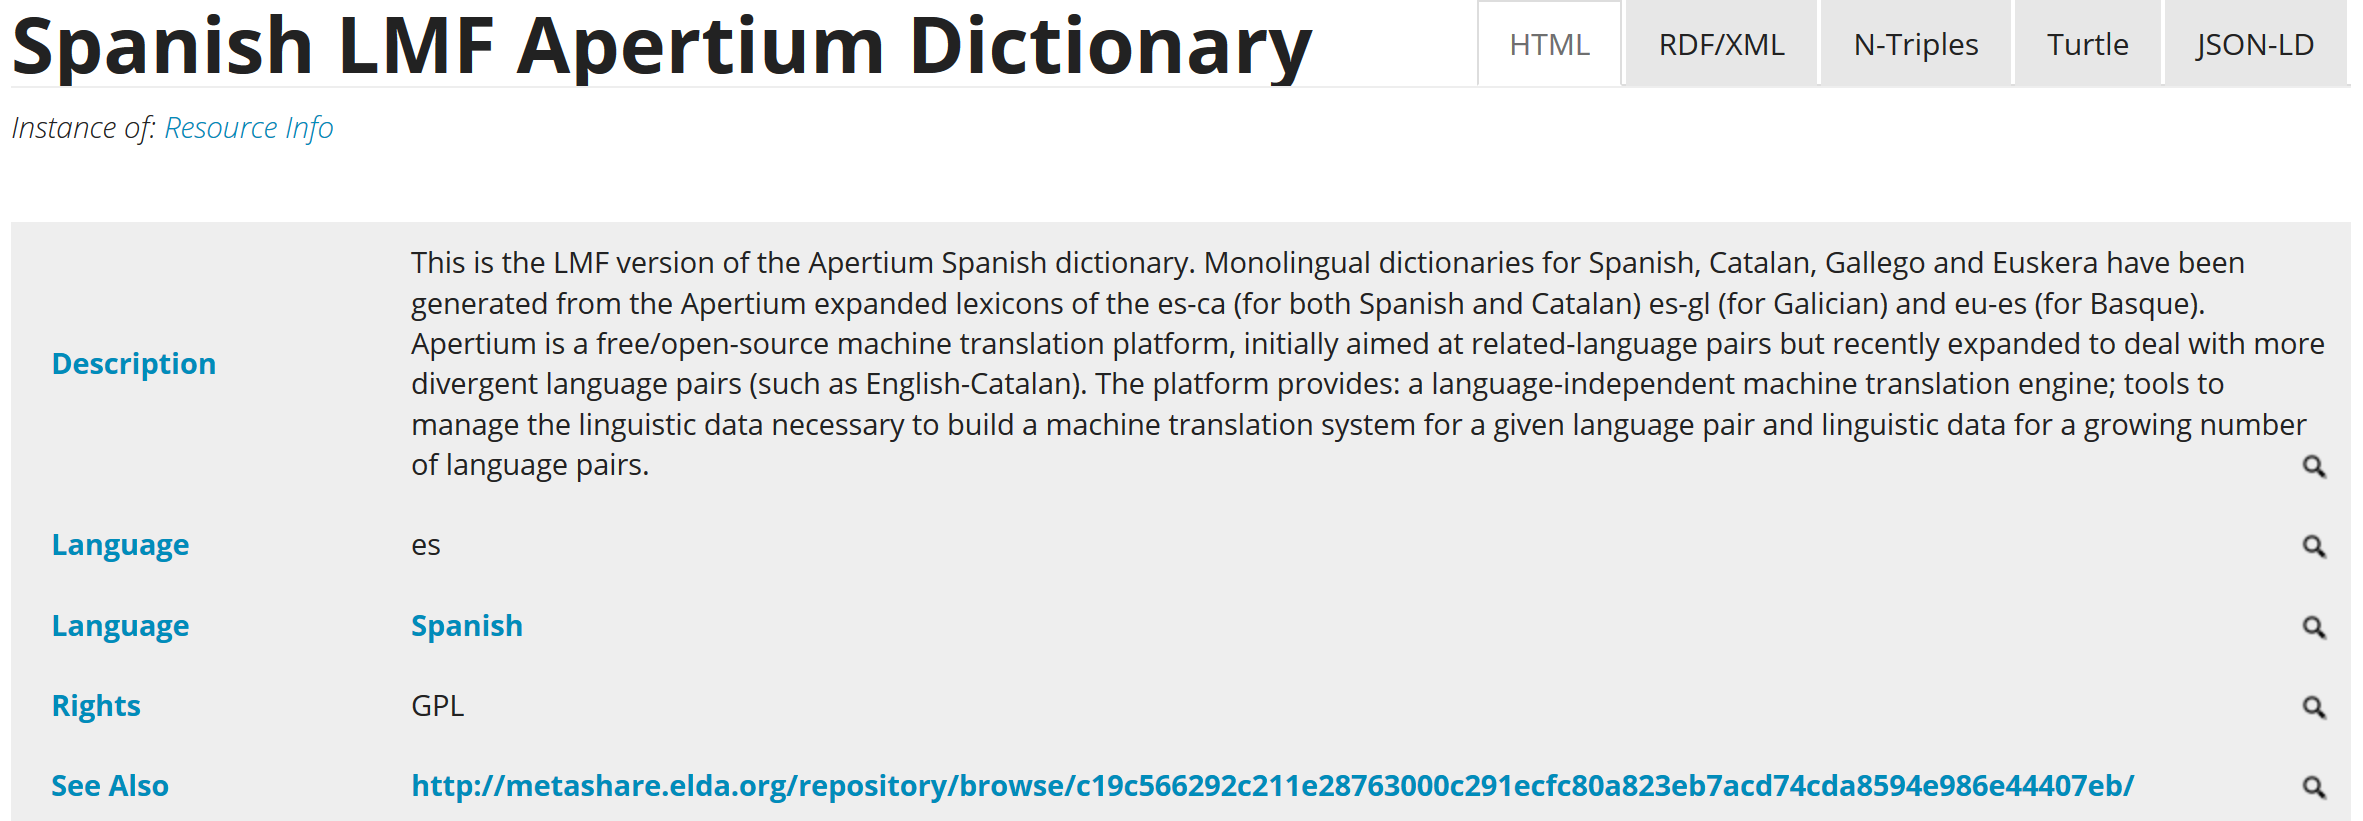
\includegraphics[width=.9\textwidth]{linghub-screenshot.png}
\caption{A screenshot of the Linghub interface\label{fig:screenshot}}
\end{figure*}

In order to enable users to quickly and easily discover datasets, we set up a 
portal for browsing the dataset. Naturally we set this up as a site that publishes
the individual records as either RDF or HTML, with the actual content delivered
to the client decided by means of content negotiation. We developed 
templates that render the RDF in a readable manner, while still appearing close
to the data so that users would get a consistent view of a dataset record even
if it came from a different original source and hence had very different
properties.
In addition, we provide a 
number of mechanisms by which users and automated agents can discover a dataset.
For users, we allowed resources to be discovered by means of faceted browsing by
allowing users to select properties and their values. We fixed the list of
properties in advance to those that have been harmonized so as to not overload
the user with choices for properties that only occur for a few datasets and also
to enable the compilation of indexes to speed up the page load. In addition the
front page of Linghub contains a free-text search engine allowing the users to
query fields by a property. This free-text search engine is powered by a
separate index which includes not only the text of data properties but also the
labels of URIs which appear as the value of object properties. 
Machine based agents may access
the endpoint by means of SPARQL querying, although the endpoint limits the agents
to a subset of the SPARQL query language. The goal of this is to enable constant
query-time without overloading our server. The nature of SPARQL makes it very
easy for users to write queries that are of a complexity that would not be easy
to answer. Other sites have attempted to handle this by enforcing timeouts on
SPARQL queries. In general we find this solution to be sub-optimal as it
means that queries may fail unpredictably if the server has many concurrent
connections. Instead, we limit the complexity of the queries themselves by
requiring that the triples have certain properties that can be easily answered.
These include:

\begin{enumerate}
    \item A required limit on the number of results;
    \item The property may not be a variable, thus limiting the number of
        results;
    \item The query must be a 'tree' in that every triples should be connected
        from a single root node.
\end{enumerate}

Furthermore, the SPARQL endpoint also by default returns SPARQL-Json
results\cite{}, so that the results may be easily applied. This is based on the
fact that many clients, notably client-side Javascript in browsers, will not
accept XML due to security concerns. Other clients may still obtain SPARQL-XML
by supplying the appropriate header or parameter in the query.

\section{Using Linghub}

In order to evaluate the practicality of Linghub as a system for finding
language resources, we wanted to identify users who were searching for languages
resources. To this end, we used \emph{Corpora List} a mailing list used by many
researchers in corpus linguistics to discuss corpora. In particular, we looked
at three queries from users.

\textquote[Thapelo J. Otlogetswe, Feb. 5th
2015\footnote{\url{http://mailman.uib.no/public/corpora/2015-February/021993.html}}]{[...] desparately needs an Igbo corpus.}

Igbo is a language of Nigeria and Equatorial Guinea and is identified with the
language code {\tt ibo}. Simply typing ``Igbo'' into the search interface of
Linghub finds a number of resources that could be used. For many of these
resources Igbo is the \emph{subject}. Although, there is a language property
some sources decided not to use this Dublin Core category. In addition these
resources are marked with a \emph{type} that is mapped to the META-SHARE {\tt
corpus} individual even though the resources do not originate from META-SHARE
due to our harmonization. We can search for
both language and subject with the following query:

\begin{verbatim}
SELECT ?resource WHERE {
 ?resource
   dct:language iso639:ibo |
   dc:subject "Igbo" ;
   dct:type metashare:corpus .
}
\end{verbatim}

\textquote[Márton Makrai, Feb. 24th
2015\footnote{\url{http://mailman.uib.no/public/corpora/2015-February/022103.html}}]{I
am looking for a Lithuanian gigaword corpus for a research project.}

Finding a corpus for a European language such as Lithuanian is generally not a
challenge, however this user also has the requirement that the resource has over
one billion words. We can easily use the META-SHARE properties to return the
user a list of corpora with their associated sizes, as follows:

\begin{verbatim}
SELECT ?resource ?size WHERE {
  ?resource
    ms:corpusInfo [
      ms:languageInfo [
        dct:language iso639:lit ;
        ms:sizePerLanguage [
          ms:size ?size ;
          ms:sizeUnit ms:words
        ]
      ]
    ] .
}
\end{verbatim}
      
\textquote[Md. Hasanuzzaman, Feb. 16th
2015\footnote{\url{http://mailman.uib.no/public/corpora/2015-February/022044.html}}]{I
    am looking for freely available geotagged tweets collection for research
purpose.}

Several of the search terms here are unfortunately not found anywhere in our
data, namely `geotagged' and `tweets' so...



\section{Conclusion}

Linghub is a new site that collects data from a large number of sources and
makes it queriable through a common mechanisms. Furthermore, the data has not
only been converted to RDF it has also been homogenized and linked to other
bubbles in the Linguistic Linked Open Data Cloud. As such, this resource is
likely to pay a pivotal role in enabling not only humans but also software
agents to find new resources and use them for applications in natural language
processing and artificial intelligence.

\section*{Acknowledgments}

%\\
%  {\bf Victor Rodr\'iguez Doncel, Daniel Vila-Suero}\\
%  {\bf Jorge Gracia} \\
%  Universidad Polit\'ecnica de Madrid \\
%  Madrid, Spain \\
%  {\scriptsize\tt\{vrodriguez, dvila, jgracia\}@fi.upm.es} \\\And
%  Luca Matteis, Roberto Navigli \\
%  University of Rome, La Sapienza \\
%  Rome, Italy \\
%  {\scriptsize\tt \{matteis, navigli\}@di.uniroma1.it} \\
%  {\bf Andrejs Abele, Gabriela Vulcu}\\
%  {\bf Paul Buitelaar} \\
%  Insight Centre, National University of Ireland\\
%  Galway, Ireland \\
%  {\scriptsize\tt \{andrejs.abele, gabriela.vulcu,}\\
%  {\scriptsize\tt paul.buitelaar\}@insight-centre.org} \\}
 
%LingHub was made possible due to significant help from a large number of people,
%in particular we would like to thank the following people: Benjamin Siemoneit
%(Bielefeld University), Tiziano Flati (University of Rome, La Sapienza), Martin
%Br\"ummer (University of Leipzig), Sebastian Hellmann (University of Leipzig),
%Bettina Klimek (University of Leipzig), Penny Labropolou (IEA-ILSP), Juli
%Bakagianni (IEA-ILSP), Stelios Piperidis (IEA-ILSP), Nicoletta Calzolari
%(ILC-CNR), Riccardo del Gratta (ILC-CNR), Marta Villegas (Pompeu Fabra),
%N\'uria Bel (Pompeu Fabra) and Christian Chiarcos (Goethe-University Frankfurt).
%
%+Asun

\bibliographystyle{abbrv}
\bibliography{../linghub-acl15}

\end{document}
